\documentclass[conference]{IEEEtran}
\IEEEoverridecommandlockouts
% The preceding line is only needed to identify funding in the first footnote. If that is unneeded, please comment it out.
\usepackage{cite}
\usepackage{amsmath,amssymb,amsfonts}
\usepackage{algorithmic}
\usepackage[pdftex]{graphicx}
\usepackage{textcomp}
\usepackage{xcolor}
\usepackage{kotex}
\usepackage{href-ul}
\usepackage{float}
\def\BibTeX{{\rm B\kern-.05em{\sc i\kern-.025em b}\kern-.08em
    T\kern-.1667em\lower.7ex\hbox{E}\kern-.125emX}}
\begin{document}

\newcommand{\libpng}{\textbf{libpng}}
\newcommand{\Eigen}{\textbf{Eigen}}

\newcommand{\eg}{\textbf{eg}}
\newcommand{\egExceptions}{\textbf{egExceptions}}
\newcommand{\egGeometry}{\textbf{egGeometry}}
\newcommand{\egLoader}{\textbf{egLoader}}
\newcommand{\egMath}{\textbf{egMath}}
\newcommand{\egMethods}{\textbf{egMethods}}
\newcommand{\egOperators}{\textbf{egOperators}}
\newcommand{\egProcessing}{\textbf{egProcessing}}
\newcommand{\egTrace}{\textbf{egTrace}}
\newcommand{\egTypes}{\textbf{egTypes}}

\newcommand{\imgascii}{\textbf{img2ascii}}
\newcommand{\tone}{\textbf{tone}}
\newcommand{\structure}{\textbf{structure}}

\title{AAC(Ascii Art Converter)\\ \vspace{1em}
{\large 2023 2학기, CSE2035/AIE2051 \\ 서강대학교 \\} \vspace{0.5em}
{
\includegraphics[width=1.5cm]{./sogang_university_logo.png}}
{\large ~\\~}
{\large \\ 기말 프로젝트 \\ Team: No More Double \\ \vspace{-1em}\href{https://github.com/arduinocc04/AAC}{https://github.com/arduinocc04/AAC}}}
\author{\IEEEauthorblockN{1\textsuperscript{st} 조다니엘}
\IEEEauthorblockA{\textit{컴퓨터공학과} \\
\textit{서강대학교} \\
danielcho@sogang.ac.kr}
\and
\IEEEauthorblockN{2\textsuperscript{nd} 박준영}
\IEEEauthorblockA{\textit{컴퓨터공학과} \\
\textit{서강대학교} \\
sparkjy18@sogang.ac.kr}}

\begin{figure}
    \hspace{2.25em}
    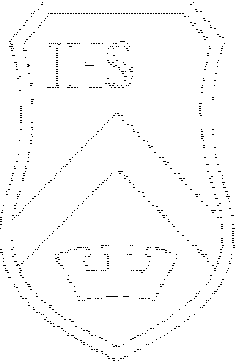
\includegraphics[width=0.75\paperwidth]{ascii_logo_1.pdf}
    \end{figure}

\maketitle

\begin{abstract}
AAC(Ascii Art Converter)는 png 이미지 파일을 아스키 아트로 변환하여 출력하는 프로그램이다.
이미지 변환 방식은 크게 tone-based 방식과 structure-based 방식으로 나뉜다.
tone-based 방식은 이미지의 각 픽셀의 rgba 값을 읽어들인 후 red, green, blue 값의 평균으로 픽셀의 밝기를 결정하여 색조 이미지를 회색조로 변환한다.
이후 픽셀의 밝기 정도에 따라 그에 해당하는 아스키 문자로 픽셀을 변환하여 출력한다.
structure-based 방식은 이미지를 회색조로 변환한 뒤 convolution 연산을 활용한 edge-detection 알고리즘을 적용하며, morphology 또는 Gaussian-blur 연산을 적용하여 정제된 결과를 얻는다.
이후 Suzuki 알고리즘을 사용하여 외곽선을 추출한 후 외곽선의 곡선을 선분으로 분할하여 이미지를 벡터화한다.
최종적으로 벡터화된 이미지를 픽셀 덩어리로 분할한 다음 덩어리별로 log-polar 히스토그램을 얻고, Bhattacharyya 거리를 이용해 가장 유사한 아스키 문자를 선택하여 출력한다.
이후 simulated annealing 기법을 이용해 이미지가 아스키아트로 잘 표현되도록 이미지를 변형시키며, 더이상 변형되지 않을 경우 종료한다.
\end{abstract}

\section{동기}
\begin{description}
    \item[박준영]: YouTube에서 접했던 donut.c\cite{b1} 아스키 아트를 보고 비슷하게 이미지 변환을 구현해 보고자 시작하였다.
    \item[조다니엘]\hspace{1em}: AAC이라는 마음이 마음에 들었다.
\end{description}

\section{프로젝트 구조}

\subsection{\eg}

\eg는 오픈 소스 라이브러리인 \libpng와 \Eigen을 사용하여 구현한 라이브러리이다.
\eg는 이미지 변환에 필요한 연산을 담당하는 \egGeometry, \egMath, \egMethods, \egOperators, \egProcessing, \egTrace와 그 밖의 이미지 입출력, 타입 정의, 에러 핸들링을 담당하는 \egLoader, \egTypes, \egExceptions로 구분된다.

\subsubsection{\egLoader}

\egLoader 에는 png 파일을 읽고, 저장하는데 도움을 주는 \libpng를 이용하여 png 이미지 파일의 가로, 세로 및 rgba 값을 읽어들인 다음 각각 텐서의 원소로 저장한다.
또한 \Eigen 텐서 형태로 저장되어 있는 Image를 다시 png 파일로 export하는 기능이 내장되어 있다.

\subsubsection{\egMethods}

\egMethods는 지원 가능한 이미지 연산, 변환 방법을 enum 타입으로 정의한 파일이다.
대표적으로 색조 변환, blur, 윤곽선 추출 등이 있다.

\subsubsection{\egMath}

\egMath는 edge-detection에 활용되는 convolution 연산, 행렬 간의 거리를 비교하는 RMSE, shape-context, log-polar 좌표계 변환 연산, 히스토그램 간의 거리를 비교하는 Bhattacharyya 연산이 포함되어 있다.

\subsubsection{\egGeometry}

\egGeometry는 시계/반시계 방향을 판단하는 ccw() 함수 및 점과 선분 사이의 거리를 계산하는 distSegDot() 함수, 내적 및 외적, 유클리드 좌표계의 거리와 log-polar 좌표계의 거리를 계산하는 함수들이 내장되어 있다. 

\subsubsection{\egProcessing}

\egProcessing은 이미지 처리와 관련된 전반적인 구현이 모두 포함되어 있다.
색조 이미지를 회색조로 변환하는 cvtGray(),
외곽선을 추출하는 getEdge(),
blur 처리를 담당하는 blur(),
grassfire 알고리즘을 활용하여 중심선을 추출하는 extractCenterline(),
0과 255 사이를 벗어나는 밝기 값을 범위 안으로 축소하는 saturate(),
일정 역치를 벗어나는 이미지의 명도 픽셀 값을 표시하는 markOutlier(),
binary 이미지의 0과 1값을 반전시키는 reverse(),
이미지 morphology 연산에 활용하기 위하여 구현한 erode() 및 dilate(),
Suzuki 알고리즘을 이용하여 외곽선을 추출하는 getContours(),
\textbf{개발하는 대로 계속 수정해 주세요~}

\subsubsection{\egTrace}

\egTrace는 distSegDot() 등 곡선을 선분으로 분할하는 함수를 사용하여 이미지의 윤곽선을 여러 선분으로 잘게 잘라 벡터화한다.

\subsubsection{\egTypes}

\egTypes에는 프로젝트에서 사용하기 위해 새롭게 정의한 타입들의 정보를 한데 모아 놓았다.

\subsubsection{\egOperators}

\egOperators에는 픽셀의 x좌표, y좌표를 각각 더하고 빼거나 부호를 반전할 수 있도록 연산자 오버로딩을 정의해 놓았다.

\subsubsection{\egExceptions}

\egExceptions는 프로그램을 실행 중에 오류가 발생하면 에러 코드를 throw하고 작동을 멈춤으로써 프로그램의 undefined behavior를 방지하는 역할을 한다.

\subsection{\imgascii}

\imgascii는 \eg 라이브러리를 바탕으로 이미지를 아스키 아트로 변환하는 과정을 기술한 소스코드이다.
tone-based 방식으로 변환하는 \tone과 structure-based 방식으로 변환하는 \structure로 나뉜다.

\subsubsection{\tone}
tone-based 방식 변환은 회색조 변환 단계 이후 각 픽셀별 red, blue, green 값의 평균을 이용하여 밝기를 추출하고, 해당 밝기의 정도에 따라 문자를 선택하여 출력한다.

\subsubsection{\structure}

\section{프로그램의 동작}

이번 절에서는 structure-based 방식의 이미지 변환을 설명한다.

\subsection{이미지 파일의 입력}

이미지 파일을 입력받는다. 이미지 파일의 형식이 png인지 확인하고, 형식에 맞지 않는 이미지 파일은 오류를 띄운다.
이는 \egLoader에 구현된 PNG 클래스에서 일어나는 일이며, 특히 openImage() 메서드...

\subsection{이미지 전처리}

\subsubsection{회색조 변환}

색조 이미지의 r, g, b값을 평균내서 회색조 이미지로 변환한다.

\subsubsection{윤곽선 추출}

회색조로 변환된 이미지의 윤곽선을 추출한다.

\subsubsection{Blurring or Morphology}

Gaussian-blur 또는 dilate, erode 연산을 이용해 노이즈를 줄인다.

\subsubsection{binary 변환}

이미지를 공백에 해당하는 0과 선에 해당하는 1로 표현하여 2차원 행렬에 저장한다.
일정 역치 이상 

\subsubsection{외곽선 추출}
Suzuki의 알고리즘\cite{suzuki}을 이용하여 외곽선을 추출한다.


\subsubsection{점의 집합을 선분으로}
suzuki의 알고리즘을 이용하면 이차원 행렬의 각 점이 어떤 외곽선에 속해있는지를 알아낼 수 있다.
이를 바탕으로 실제 외곽선을 구해내려면, 같은 외곽선에 있는 점을 시계방향 또는 반시계방향으로 정렬해야한다.
이를 위해, 알고리즘을 자체 제작하였다. 
\begin{enumerate}
    \item 왼쪽 위$(0, 0)$ 부터 오른쪽 아래$(H, W)$ 방향으로 행렬의 각 원소를 검사한다. \label{taecho}
    \item 만약 그 픽셀의 값이 이전에 봤던 값이거나 0 이라면 \ref{taecho}로 돌아간다.
    \item 자신과 인접한 왼쪽 아래에 있는 픽셀부터 시계 반대방향으로 자신과 같은 외곽선에 속한 픽셀을 찾는다. 없다면 \ref{taecho}로 돌아간다. \label{find1}
    \item 이후 연결된 픽셀을 순차적으로 탐색하여, 연결된 픽셀이 더이상 없을때까지 스택에 픽셀의 좌표를 넣는다.
    \item 스택을 뒤집는다.
    \item \ref{find1}에서 발견했던 픽셀의 시계 반대방향 순서로 다음에 있는 픽셀부터, 시계 반대방향 순서로 탐색을 시작한다.
    만약 기존에 방문한 픽셀 밖에 없거나, 같은 외곽선에 속한 픽셀을 찾지 못 한다면 \ref{taecho}로 돌아간다.
    \item 이후 연결된 픽셀을 순차적으로 탐색하여, 연결된 픽셀이 더이상 없을때까지 스택에 픽셀의 좌표를 넣는다. 이후 \ref{taecho}로 돌아간다.
\end{enumerate}
\begin{figure}
    \centering
    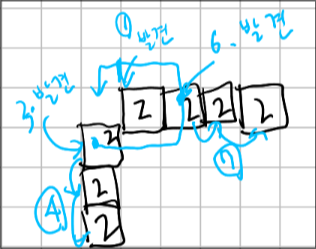
\includegraphics[width=6cm]{algo.png}
    \caption{점의 집합을 시계방향 또는 시계 반대방향으로 정렬하는 알고리즘}
\end{figure}
이후, 간단한 그리디 알고리즘을 이용하여 점들을 선분으로 근사한다.
선분$\overline{A_1A_2}$와 점 $P$ 사이의 거리는 식 \ref{eq:distDotSeg}\로 정의한다.
\begin{equation}
    \begin{cases}
        \overline{A_1P} & \text{If } (A_2 - A_1)\cdot (P - A_1) \leq 0 \\
        \overline{A_2P} & \text{If } (A_1 - A_2)\cdot(P - A_2) \leq 0 \\
        \frac{|(P - A_1)\times (A_2 - A_1)|}{\overline{A_1A_2}} & \text{otherwise}

    \end{cases}
    \label{eq:distDotSeg}
\end{equation}
시계 방향 또는 시계 반대 방향으로 정렬된 점들의 배열 $A$가 주어졌을 때, 어떤 $i < j$인 음이 아닌 정수 $i, j$가 존재하여,
선분 $\overline{A_iA_j}$와 점 $A_k$($i < k < j$)의 거리가 $\sqrt 2 \approx 1.42$ 이하라면, $i$에서 $j$번째까지의 점들을 선분으로 근사했다고 말할 수 있을 것이다.
이를 배열 앞쪽부터 보면서 선분으로 모을 수 있을때는 항상 모으고, 아니면 빠르게 포기하고 새로운 선분을 만들기 시작한다.
\subsection{이미지 최적화}
\subsubsection{선분을 그리드로 분할}
Cohen-Sutherland 알고리즘\cite{cohen-sutherland}을 사용하여 기다란 선분을 그리드마다 분할해둔다.

\subsubsection{simulated annealing}
임의의 정점을 조금씩 움직여보면서 Bresenham's line algorithm\cite{bresenham-line}을 사용해 그림을 새로 그린다.
이후 아스키아트를 더 잘 표현하는 이미지로 변화했는지 확인한다.
주어진 그리드에 어떤 문자가 가장 잘 대응되는지는 log polar coordinate로 변환한 후 히스토그램을 만든 후,
Bhattacharyya 거리를 비교하여 판단한다.
자세한 내용은 \cite{st-ba-ascii-art}로..


\section{프로젝트 진행 과정}

프로젝트의 첫 계획은 이미지를 아스키 아트로 변환하는 프로그램과 변환된 아스키 아트를 출력하는 프로그램 두 가지를 결합하는 형식이었다.
그러나 Qt로 뷰어를 구현하는 과정은 번잡하고 지루하였기 때문에 아스키 아트 변환에만 집중해서 프로젝트를 진행하기로 결정하였다.
방식을 일반적으로 널리 알려지고 구현 난도도 낮은 tone-based 방식과 구현 난이도가 높지만 훨씬 만족스러운 결과를 도출하는 structure-based 방식으로 나누어 각자 구현하기로 하였다.
처음에는 libpng를 제외하고 아무런 오픈 소스 라이브러리를 사용하지 않으려고 하였기 때문에 이미지를 쉽고 빠르게 입출력할 수 있는 사용자 라이브러리를 만들었다.


\section{사용 방법}
\begin{enumerate}
\item \begin{verbatim}sudo pacman -S libpng eigen\end{verbatim}
\item \begin{verbatim}git clone https://github.com/arduinocc04/AAC\end{verbatim}
\item \begin{verbatim}cd AAC\end{verbatim}
\item \begin{verbatim}./install.sh\end{verbatim}
\item \begin{verbatim}cd build \end{verbatim}
\item \begin{verbatim}img2ascii/structure/sa-structure non-hangul-images IMAGE_FILE\end{verbatim}
\end{enumerate}


\begin{thebibliography}{00}
\bibitem{b1} % donut.c
\bibitem{suzuki} % https://www.sciencedirect.com/science/article/abs/pii/0734189X85900167
\bibitem{monotone-chain} % https://en.wikibooks.org/wiki/Algorithm_Implementation/Geometry/Convex_hull/Monotone_chain
\bibitem{grassfire} % https://en.wikipedia.org/wiki/Grassfire_transform
\bibitem{cohen-sutherland} % https://en.wikipedia.org/wiki/Cohen%E2%80%93Sutherland_algorithm
\bibitem{st-ba-ascii-art} % https://dl.acm.org/doi/10.1145/1778765.1778789
\bibitem{bresenham-line} % https://en.wikipedia.org/wiki/Bresenham%27s_line_algorithm
\bibitem{}
\end{thebibliography}

\end{document}
